\documentclass[12pt,notitlepage]{article}

\usepackage[utf8]{inputenc}
\usepackage[english]{babel}

% https://tex.stackexchange.com/questions/11778/modifying-everydisplay-causes-the-align-environment-to-stop-working
\let\displaystyle\textstyle

\usepackage[
backend=biber,
giveninits=true,
url=false,
isbn=false,
backref=true,
style=alphabetic,
sorting=ynt,
block=none,
maxcitenames=3,
maxbibnames=100,
]{biblatex}
%
\addbibresource{refs.bib}

%\usepackage{natbib} % bibtex
%\let\cite\citep


\usepackage{amsmath, amsfonts, amssymb, mathtools}
\usepackage[svgnames]{xcolor}
\usepackage{datetime2}
\usepackage[
	colorlinks=true, 
	citecolor={DarkRed}, urlcolor={DarkBlue}, linkcolor={DarkBlue},
]{hyperref}


% https://tex.stackexchange.com/questions/3802/how-to-get-doi-links-in-bibliography
% \usepackage{doi}

% 
\usepackage[version=4]{mhchem}
\mhchemoptions{font=sf}

% http://mirrors.ibiblio.org/CTAN/macros/latex/contrib/siunitx/siunitx.pdf
\usepackage{siunitx}


\usepackage{fullpage}

% Paragraph spacing
\usepackage{parskip}
%\usepackage{enumitem}

\usepackage{xspace}

\usepackage{graphicx}
\graphicspath{{../code/}{../images/}}
\DeclareGraphicsExtensions{.pdf,.eps,.png}

% https://tex.stackexchange.com/questions/202046/width-of-the-caption-of-a-figure
% https://tex.stackexchange.com/questions/29039/how-to-limit-the-figure-caption-width
% https://tex.stackexchange.com/questions/822/change-the-font-of-figure-captions
\usepackage[margin=10px,font={small}]{caption}
% https://tex.stackexchange.com/questions/25879/multiple-captions-for-a-single-figure
\usepackage{subcaption}


% http://www.texfaq.org/FAQ-ftnsect
\usepackage[stable]{footmisc}

% https://tex.stackexchange.com/questions/20792/how-to-superimpose-latex-on-a-picture
\usepackage[percent]{overpic}

%\usepackage{epstopdf}

% Tables (the order matters here)
\usepackage{makecell}
\usepackage{booktabs}
\usepackage{arydshln}

% https://tex.stackexchange.com/questions/109467/footnote-in-tabular-environment
\usepackage{footnote}
\makesavenoteenv{tabular}
\makesavenoteenv{table}

% https://tex.stackexchange.com/questions/10130/use-the-values-of-title-author-and-date-on-a-custom-title-page
\usepackage{authoraftertitle}

% https://en.wikibooks.org/wiki/LaTeX/Footnotes_and_Margin_Notes#Margin_Notes
\usepackage{marginnote}

% For editing purposes:
%\usepackage[margin=10pt]{geometry}

% https://latex.org/forum/viewtopic.php?t=10456
\usepackage{titlesec}
\titleformat{\subsubsection}[runin]% runin puts it in the same paragraph
{\normalfont\bfseries}% formatting commands to apply to the whole heading
{\thesubsubsection}% the label and number
{}% space between label/number and subsection title
{}% formatting commands applied just to subsection title
[.]% punctuation or other commands following subsection title



% https://bitbucket.org/goodnightmath/covariance/src/master/tex/main.tex

%%%%%%%%%%%%%%%%%%%%%%%%%%%%%%%%%%%%%%%%%%%%%%%%%%%%%%%%%%%%%%%%%%%%%%%%%%%%%%%
\providecommand{\TODO}[1]{\textrm{\color{red}TODO: #1}}

% http://tex.stackexchange.com/a/106577/44073
\usepackage{ifthen}
\newcounter{todoindex}\setcounter{todoindex}{0}
\newcommand\ADDTODO[1]{%
	\addtocounter{todoindex}{1}%
	\expandafter\gdef\csname todo\roman{todoindex}\endcsname{#1}%
	%\expandafter\csname todolabel\roman{todoindex}\endcsname
	\label{todolabel\roman{todoindex}}
}
\renewcommand\TODO[1]{%
	{%
		\ADDTODO{#1}%
		{\textrm{\color{red}TODO(\arabic{todoindex}): #1}}%
	}%
}
\newcommand\CHECK[1]{%
	\ADDTODO{CHECK CLAIM: {#1}}%
	{\color{toverify}#1}%
	\smash{\marginnote{\text{\color{red}*}}}%
}
\newcounter{indextodo}
\newcommand{\SHOWTODOS}{%
	\setcounter{indextodo}{0}%
	\begin{enumerate}
	\item[{\color{red} TODOs:}]
	\whiledo{\value{indextodo} < \value{todoindex}}{%
		\addtocounter{indextodo}{1}%
		\item[\color{red}\arabic{indextodo}.]
		p.\pageref{todolabel\roman{indextodo}}.
		%
		\csname todo\roman{indextodo}\endcsname
	}%
	\end{enumerate}
}
%%%%%%%%%%%%%%%%%%%%%%%%%%%%%%%%%%%%%%%%%%%%%%%%%%%%%%%%%%%%%%%%%%%%%%%%%%%%%%%



\renewcommand{\d}{\mathrm{d}}
\newcommand{\ddt}{\frac{\d}{\d{t}}}

\newcommand{\TEXT}[1]{\quad\text{#1}\quad}
\newcommand{\with}{\text{$\,{:}\,$}}

\newcommand{\cbra}[1]{{\ensuremath{\color{gray}{#1}}}}
\newcommand{\signal}[1]{{{\cbra{\langle}\ce{#1}\cbra{\rangle}}}}
\newcommand{\protein}[1]{{{\cbra{(}\ce{#1}\cbra{)}}}}
\newcommand{\promoter}[1]{{{\cbra{[}\ce{#1}\cbra{]}}}}

% https://tex.stackexchange.com/questions/543953/arrow-with-blunted-end-head-in-math-mode
\newcommand{\act}{\ {\ensuremath{\mathbin{\to}}}\ }
\newcommand{\rep}{\ {\ensuremath{\mathrel{\raisebox{-.3ex}{\rotatebox{90}{\scalebox{1}[1.2]{$\bot$}}}}}}\ }

\def\[#1\]{\begin{align}#1\end{align}}

% https://tex.stackexchange.com/questions/114113/how-to-label-text-with-equation-number
\newcommand{\eqnum}{\leavevmode\hfill\refstepcounter{equation}\textup{{(\theequation)}}}

\newcommand{\starlink}[1]{\textsuperscript{\makebox[0pt]{\href{#1}{\color{white}$\star$}}}}

\newcommand{\hh}[1]{{\color{Purple}#1}}
\newcommand{\ra}[1]{{\color{Blue}#1}\marginnote{\TODO{review}}}


\title{DRAFT: NCT}
\author{RA}
\date{\today}
\newcommand{\linktodoc}{http://bit.ly/}




\begin{document}

\maketitle

\section{NCT models}

Abbreviations:
FG-nups = FG-nucleoporins;
NCT = nucleocytoplasmic transport;
NPC = nuclear pore complex;
ODE = ordinary differential equations.

\subsection{GSR'03 model of NCT} \label{s:GSR03}

\subsubsection*{Ran gradient} \label{s:GSR03:Ran}

First we implement
the ``minimal Ran gradient system'' from 
\cite{GoerlichSeewaldRibbeck2003}.
%
%
The equations are shown in
Table~\ref{t:GSR-Ran}
and
the constants are collected in 
Table~\ref{t:GSR-const}.
%
%
The ``dynamic capacity'' \ce{Ex}
is an optional maximal steady-state (positive) flux
of nuclear \ce{Ran.GTP} to cytoplasmic \ce{Ran.GDP},
which we determine using the additional equation \eqref{e:Ex}.
%
%
The fluxes 
are in units of concentration/time (\si{\micro M \per s}).
%
The ones across the nuclear boundary
have positive sign when exiting the nucleus
and are normalized to the nuclear volume.
%
Thus,
the \emph{amount} exiting the nucleus per unit of time is
$\ce{flux} \times V_\text{nuc}$.

%

Simulating the ODE
across the scenarios of 
\cite{GoerlichSeewaldRibbeck2003}
we obtain 
results that are sufficiently close
to the original,
see Table~\ref{t:GSR-Ran-Runs}.
%
%
Importantly,
a 1000-fold nuclear enrichment of \ce{Ran.GTP}
is sustained in steady-state.

%

Code:
\href{https://github.com/numpde/nct1/tree/d56d16f/code/20210225-GSR/v1}{d56d16f/code/20210225-GSR/v1}

%

\subsubsection*{Coupling to transport} \label{s:GSR03:Imp}

A coupling of the Ran gradient
to 
importin--cargo transport
was proposed in 
\cite[Fig.~6A]{GoerlichSeewaldRibbeck2003}.
%
We formulate a version of it in 
Table~\ref{t:GSR-ImpB}.

%

With the constants from Table~\ref{t:GSR-ImpB-const},
the steady-state of the model
(reached after some $10^4 \si{. s}$)
is reported in Fig.~\ref{f:GSR-v2}.
%
Nuclear
accumulation of free cargo
is over 20-fold.
%
%
Sensitivity analysis shows
that, in relative terms,
the final nuclear concentration of free cargo
depends 
most strongly
on
$k_\text{knockoff}$
(and the volume of the nucleus).
%
Doubling $k_\text{knockoff}$ almost doubles 
the nuclear concentration.
%


Code:
\href{https://github.com/numpde/nct1/tree/2a2199d/code/20210225-GSR/v2}{2a2199d/code/20210225-GSR/v2}


%

\TODO{?
\cite{Catimel2001} and \cite{RiddickMacara2005}
discuss
the reaction 
\ce{Imp$\beta$ . Cargo <=> Imp$\beta$^* . Cargo}
}




\subsection{NPC as compartments} \label{s:GSR03-redux}

It has been observed \TODO{ref}
that 
certain transportins accumulate 
inside the NPCs
as they bind to the FG-nups.
%
%
They might potentially shuttle
the cargo across the pore
without leaving the pore themselves,
like a conveyor belt.
%
%
To account for this
we propose
a three-compartment model
with cytoplasm, nucleus
and
the nuclear envelope 
(potentially including some perimembrane space)
as the three compartments.
%
%
The crux is that the nuclear envelope, 
having small volume, 
has a high concentration of NPCs.
%
%
The unoccupied NPC space 
is called \ce{NPC_{vacant}}.
%
%
At the nuclear envelope we posit the reactions
\begin{subequations}
\[
	\ce{Imp$\beta$_i + NPC_{vacant} & <=> Imp$\beta$.NPC}
	\\
	\ce{Cargo.Imp$\beta$_i + NPC_{vacant} & <=> Cargo.Imp$\beta$.NPC}
	\\
	\ce{Cargo_i + Imp$\beta$.NPC & <=> Cargo.Imp$\beta$.NPC}
\]
\end{subequations}
where $i$ can be ``cytoplasmic'' or ``nuclear''.
%
%
This envelope compartment
is in diffusive exchange with 
the cytoplasm (for $i = \text{cyt}$)
and
the nucleus (for $i = \text{nuc}$).
%
%
In both, we also allow 
\[
	\ce{Cargo + Imp$\beta$ & <=> Cargo.Imp$\beta$}
	.
\]
%
%
For simplicity,
we assume 
\ce{RanGTP} and \ce{RanGDP} 
are maintained at fixed concentrations
and are only relevant at the envelope,
where we have
\begin{subequations}
\[
	&
	\text{cargo knockoff:}
	&
	\ce{
		RanGTP_{nuc} + Cargo.Imp$\beta$.NPC
		& ->
		Cargo + RanGTP.Imp$\beta$.NPC
	}
	%
	\\
	%
	&
	\text{GTP hydrolysis: \hspace{-1cm}}
	&
	\ce{
		RanGTP.Imp$\beta$.NPC 
		& ->
		RanGDP_{cyt} + P + Imp$\beta$.NPC 
	}
	.
\]
\end{subequations}

%

Under reasonable assumptions on the kinetic constants,
the steady state of this model
predicts some 10-fold accumulation
of free cargo in the nucleus.
%
Meanwhile,
the concentration of total \ce{Imp\beta}
is roughly inversely proportional
to the volume of the envelope compartment
(keeping the total \ce{NPC} amount constant).

Code:
\href{https://github.com/numpde/nct1/tree/main/code/20210403-StickyPore/b_onestage_nct}{here}




\begin{table} \small
The following account for the cytoplasmic species.
%
Here,
$\ce{[\ldots]}$ abbreviates 
the (cytoplasmic) concentration of 
the complex \ce{{RanBP1} . Ran.GTP}.
%(in presence of \ce{RanGAP}, this term can be omitted).
%
%
\begin{subequations}
\[
	\label{e:Eq1}
	%
	\ddt
	[\ce{Ran.GDP}]_\text{cyt}
	& =
	\ce{F_{\ce{Ran.GDP}}} \frac{V_\text{nuc}}{V_\text{cyt}} 
	+
	\ce{GAP}
	+
	\ce{GAP_{RanBP1}}
	+
	\ce{Ex} \frac{V_\text{nuc}}{V_\text{cyt}} 
	%
	%
	\\
	\label{e:Eq2}
	%
	\ddt
	[\ce{Ran.GTP}]_\text{cyt}
	& = 
	\ce{F_{\ce{Ran.GTP}}} \frac{V_\text{nuc}}{V_\text{cyt}}
	-
	\ce{GAP}
	-
	k_\text{on}^\text{rbp}
	[\ce{{RanBP1}}] [\ce{Ran.GTP}]_\text{cyt}
	+
	k_\text{off}^\text{rbp}
	[\ce{\ldots}]
	%
	%
	\\
	\label{e:Eq3}
	%
	\ddt
	[\ce{{RanBP1} . Ran.GTP}]
	& =
	-
	\ce{GAP_{RanBP1}}
	\quad\quad\quad
	+
	k_\text{on}^\text{rbp}
	[\ce{{RanBP1}}] [\ce{Ran.GTP}]_\text{cyt}
	-
	k_\text{off}^\text{rbp}
	[\ce{\ldots}]
\]
\end{subequations}


The following account for the nuclear species.
%
Following \cite{GoerlichSeewaldRibbeck2003},
\ce{E} denotes free \ce{{RCC1}}.
%
%
\begin{subequations}
\[
	\label{e:Eq4}
	%
	\ddt
	[\ce{Ran.GDP}]_\text{nuc}
	& =
	-
	\ce{F_{\ce{Ran.GDP}}}
	+
	r_8
	[\ce{IntC}]
	-
	r_1
	[\ce{E}]
	[\ce{Ran.GDP}]_\text{nuc}
	%
	%
	\\
	\label{e:Eq5}
	%
	\ddt
	[\ce{Ran.GTP}]_\text{nuc}
	& =
	-
	\ce{F_{\ce{Ran.GTP}}}
	+
	r_4
	[\ce{IntA}]
	-
	r_5
	[\ce{E}]
	[\ce{Ran.GTP}]_\text{nuc}
	-
	\ce{Ex}
\]
\end{subequations}


The nucleotide-exchange reaction
\ce{Ran.GDP + GTP <=> Ran.GTP + GDP}
is catalyzed by \ce{{RCC1}}.
%
It is modeled as in 
\cite[Fig.~6]{KlebePrinzWittinghoferGoody1995}
/
\cite[Fig.~1]{GoerlichSeewaldRibbeck2003}
with three intermediates.
%
Note that it depends on
the availability of \ce{GDP} and \ce{GTP}.
%
%
\begin{subequations}
\[
	\label{e:Eq6}
	%
	\ddt
	[\ce{IntA}]
	& =
	-(r_4 + r_6)
	[\ce{IntA}]
	+
	r_5
	[\ce{E}] [\ce{Ran.GTP}]_\text{nuc}
	+
	r_3
	[\ce{GTP}] [\ce{IntB}]
	%
	%
	\\
	\label{e:Eq7}
	%
	%
	\ddt
	[\ce{IntB}]
	& =
	r_6 [\ce{IntA}]
	+
	r_2 [\ce{IntC}]
	-
	(r_3 [\ce{GTP}] + r_7 [\ce{GDP}])
	[\ce{IntB}]
	%
	\\
	\label{e:Eq8}
	%
	\ddt
	[\ce{IntC}]
	& =
	-
	(r_2 + r_8) [\ce{IntC}]
	+
	r_1 [\ce{E}] [\ce{Ran.GDP}]_\text{nuc}
	+
	r_7 [\ce{GDP}] [\ce{IntB}]
\]
\end{subequations}


Constraints on the total concentration:
%
%
\begin{subequations}
\[
	\label{e:Eq9}
	%
	\text{Free \ce{{RCC1}}}:
	& &
	\ce{[E]}
	& =
	\ce{{RCC1}_{total}} - (\ce{[IntA]} + \ce{[IntB]} + \ce{[IntC]})
	%
	\\
	\label{e:Eq10}
	%
	\text{Free \ce{{RanBP1}}}:
	& &
	\ce{[{RanBP1}]}
	& =
	\ce{{RanBP1}_{total}} - \ce{[{RanBP1} . Ran.GTP]}
\]
\end{subequations}


Gradient-driven fluxes from 
the nucleus to the cytoplasm:
%
%
\begin{subequations}
\[
	\label{e:Eq11}
	%
	\ce{F_{Ran.GTP}}
	& =
	D_{\ce{Ran.GTP}}
	\;
	([\ce{Ran.GTP}]_\text{nuc} - [\ce{Ran.GTP}]_\text{cyt})
	%
	\\
	\label{e:Eq12}
	%
	\ce{F_{Ran.GDP}}
	& =
	D_{\ce{Ran.GDP}}
	\;
	([\ce{Ran.GDP}]_\text{nuc} - [\ce{Ran.GDP}]_\text{cyt})
\]
\end{subequations}


\ce{RanGAP} hydrolyzes the $\gamma$-phosphate of \ce{Ran.GTP}.
%
This is more efficient
when \ce{Ran.GTP} is bound to \ce{{RanBP1}}
\cite{BischoffKrebberSmirnovaDongPonstingl1995},
reducing the IC50 seven-fold
\cite[Table~I, p.~1091]{GoerlichSeewaldRibbeck2003}.
%
%
%
\begin{subequations}
\[
	\label{e:Eq13}
	%
	\ce{GAP} 
	& = 
	k_{\ce{GAP}} [\ce{RanGAP}]
	/
	(
		1 + K_{\ce{GAP}} / [\ce{Ran.GTP}]_\text{cyt}
	)
	%
	\\
	\label{e:Eq14}
	%
	\ce{GAP_{RanBP1}} 
	& = 
	k_{\ce{GAP}}' [\ce{RanGAP}]
	/
	(
		1 + K_{\ce{GAP}}' / [\ce{{RanBP1} . Ran.GTP}]
	)
\]
\end{subequations}
%
To determine the dynamic capacity \ce{Ex}
at steady-state
we introduce
the additional equation:
\[
	\label{e:Ex}
	%
	\ddt \ce{Ex}
	=
	k_{\ce{Ex}} \, [\ce{Ran . {GTP}}]_\text{nuc},
	\quad
	k_{\ce{Ex}} := \SI{10}{s^{-2}},
	\TEXT{initial}
	\ce{Ex} := \SI{0}{\micro M . s^{-1}}
	.
\]
%
\caption{%
	The minimal Ran gradient system
	from \cite[Fig.~2]{GoerlichSeewaldRibbeck2003}.
	%
	\ce{Ex} is an additional potentially useful flux of 
	nuclear \ce{Ran.GTP} to cytoplasmic \ce{Ran.GDP},
	set by default to zero.
}
\label{t:GSR-Ran}
\end{table}


\begin{table}
\centering
\small
\begin{tabular}{c|c|c}
%	Eqn & Constants & References
%	\\
	\hline
	%
	%
	\eqref{e:Eq1}
	&
	$V_\text{nuc} = \SI{1.2}{pl}$,
	\quad
	$V_\text{cyt} = \SI{1.8}{pl}$
	& 
	\cite[Table II]{GoerlichSeewaldRibbeck2003}
	\\
	\hline
	%
	%
	\eqref{e:Eq1}
	&
	initial condition
	$[\ce{Ran . GDP}]_\text{cyt} = \SI{5}{\micro M}$
	&
	\cite[Table II]{GoerlichSeewaldRibbeck2003}
	\\
	\hline
	%
	%
	\eqref{e:Eq2}--\eqref{e:Eq3}
	&
	$k_\text{on}^\text{rbp} = \SI{0.3}{\micro M^{-1}.s^{-1}}$,
	\quad
	$k_\text{off}^\text{rbp} = \SI{4e-4}{s^{-1}}$
	&
	\cite[Supp.~Table~A]{GoerlichSeewaldRibbeck2003}
	\\
	\hline
	%
	%
	\eqref{e:Eq4}--\eqref{e:Eq8}
	&
	\makecell{
		$r_1 = \SI{74}{\micro M^{-1} . s^{-1}}$,
		\quad
		$r_8 = \SI{55}{s^{-1}}$
		\\
		$r_7 = \SI{11}{\micro M^{-1} . s^{-1}}$,
		\quad
		$r_2 = \SI{21}{s^{-1}}$
		\\
		$r_3 = \SI{0.6}{\micro M^{-1} . s^{-1}}$,
		\quad
		$r_6 = \SI{19}{s^{-1}}$
		\\
		$r_5 = \SI{100}{\micro M^{-1} . s^{-1}}$,
		\quad
		$r_4 = \SI{55}{s^{-1}}$
	}
	&
	\makecell{
		\cite[Supp.~Table~A]{GoerlichSeewaldRibbeck2003}
		\\
		\cite[Fig.~6]{KlebePrinzWittinghoferGoody1995}
	}
	\\
	\hline
	%
	%
	\eqref{e:Eq6}--\eqref{e:Eq8}
	&
	$[\ce{GTP}] = \SI{500}{\micro M}$,
	\quad
	$[\ce{GDP}] = \SI{1.6}{\micro M}$
	&
	\cite[Table II]{GoerlichSeewaldRibbeck2003}
	\\
	\hline
	%
	%
	\makecell{
		\eqref{e:Eq9} \\ \eqref{e:Eq10}
	}
	&
	\makecell{
		$\ce{{RCC1}_{total}} = \SI{0.7}{\micro M}$
		\\
		$\ce{{RanBP1}_{total}} = \SI{2}{\micro M}$
	}
	&
	\makecell{
		\cite[Supp.~Table~B]{GoerlichSeewaldRibbeck2003}
		\\
		\cite[Fig.~4]{GoerlichSeewaldRibbeck2003}
	}
	\\
	\hline
	%
	%
	\makecell{
		\eqref{e:Eq11} \\ \eqref{e:Eq12}
	}
	&
	\makecell{
		$D_{\ce{Ran . GTP}} = \SI{0.03}{s^{-1}}$
		\\
		$D_{\ce{Ran . GDP}} = \SI{0.12}{s^{-1}}$
	}
	&
	\cite[Table II]{GoerlichSeewaldRibbeck2003}
	\\
	\hline
	%
	%
	\makecell{
		\eqref{e:Eq13} \\ \eqref{e:Eq14}
	}
	&
	\makecell{
		$k_{\ce{GAP}} = \SI{10.6}{s^{-1}}$,
		\quad
		$K_{\ce{GAP}} = \SI{0.7}{\micro M}$
		\\
		$k_{\ce{GAP}}' = \SI{10.8}{s^{-1}}$,
		\quad
		$K_{\ce{GAP}}' = \SI{0.1}{\micro M}$
	}
	&
	\makecell{
		\cite[Supp.~Table~A]{GoerlichSeewaldRibbeck2003}
		\\
		\cite[Table~I]{GoerlichSeewaldRibbeck2003}
	}
	\\
	\hline
	%
	%
	\eqref{e:Eq13}--\eqref{e:Eq14}
	&
	cytoplasmic
	$[\ce{RanGAP}] = \SI{0.7}{\micro M}$
	&
	\cite[Table~II / ST~B]{GoerlichSeewaldRibbeck2003}
	% / \cite[Fig.~4]{GoerlichSeewaldRibbeck2003}
	\\
	\hline
%	%
%	%
%	\TODO{Eq}
%	&
%	$K_R = \SI{5e-4}{\micro M}$
%	&
%	\cite[Supp.~Table~A]{GoerlichSeewaldRibbeck2003}
%	\\
%	\hline
\end{tabular}
%
\caption{%
	Constants
	for the ``standard simulation condition''
	of \S\ref{s:GSR03}
	at $\SI{25}{\celsius}$.
	%
	Except for \eqref{e:Eq1},
	all species are initialized to zero at $t = 0$.
}
%
\label{t:GSR-const}
\end{table}


\begin{table}
\centering
\footnotesize
\begin{tabular}{c|c|c|c|c}
	\hline
	%
	Condition
	& 
	\makecell{
		Affected \\ parameters
	}
	&
	\makecell{
		Nuclear
		\\
		RanGTP, \si{\micro M}
	}
	&
	\makecell{
		Cytoplasmic
		\\
		RanGTP, \si{\nano M}
	}
	&
	\makecell{
		Dynamic
		\\
		capacity, \si{\micro M \per s}
	}
	%
	\\
	\hline\hline
	%
	``Standard''
	& 
	See Table~\ref{t:GSR-const} 
	&
	4.26
	(4.3)
	&
	7.75
	(7.7)
	&
	0.59 (0.60)
	%
	\\
	\hline
	%
	Omission of RanBP1
	&
	$\ce{{RanBP1}_{total}} := 0$
	&
	4.27
	(4.3)
	& 
	8.13
	(8.1)
	&
	0.59 (0.60)
	%
	\\
	\hline
	%
	200\% RCC1
	&
	\ce{{RCC1}_{total}}
	&
	3.95
	(4.0)
	& 
	7.17
	(7.1)
	&
	0.59 (0.60)
	%
	\\
	\hline
	%
	50\% RCC1
	&
	\ce{{RCC1}_{total}}
	&
	4.31
	(4.3)
	& 
	7.82
	(7.7)
	&
	0.58 (0.60)
	%
	\\
	\hline
	%
	10\% RCC1
	&
	\ce{{RCC1}_{total}}
	&
	3.59
	(3.6)
	& 
	6.50
	(6.4)
	&
	0.46 (0.48)
	%
	\\
	\hline
	%
	1\% RCC1
	&
	\ce{{RCC1}_{total}}
	&
	1.40
	(1.4)
	& 
	2.52
	(2.5)
	&
	0.075 (0.08)
	%
	\\
	\hline
	%
	GTP:GDP = 500:0
	&
	$[\ce{GDP}] := \SI{0}{\micro M}$
	&
	4.80
	(4.8)
	& 
	8.72
	(8.6)
	&
	0.59 (0.60)
	%
	\\
	\hline
	%
	GTP:GDP = 500:50
	&
	$[\ce{GDP}] := \frac{1}{10} [\ce{GTP}]$
	&
	0.98
	(0.8)
	& 
	1.76
	(1.5)
	&
	0.57 (0.58)
	%
	\\
	\hline
	%
	GTP:GDP = 500:500
	&
	$[\ce{GDP}] := [\ce{GTP}]$
	&
	0.12
	(0.12)
	& 
	0.22
	(0.21)
	&
	0.34 (0.34)
	%
	\\
	\hline
	%
	Saturating NTF2
	% Fig.~3
	&
	$D_{\ce{Ran . GDP}} := \SI{0.48}{s^{-1}}$
	&
	5.12
	(5.1)
	& 
	9.32
	(9.2)
	&
	2.18 (2.2)
	%
	\\
	\hline
	%
	No NTF2
	&
	$D_{\ce{Ran . GDP}} := D_{\ce{Ran . GTP}}$
	&
	2.55
	(2.5)
	& 
	4.60
	(4.5)
	&
	0.15 (0.16)
	%
	\\
	\hline
	%
	200\% RanGAP
	&
	$[\ce{RanGAP}]$
	&
	4.27
	(4.3)
	& 
	3.95
	(3.9)
	&
	0.59 (0.60)
	%
	\\
	\hline
	%
	50\% RanGAP
	&
	$[\ce{RanGAP}]$
	&
	4.26
	(4.3)
	& 
	14.9
	(14)
	&
	0.59 (0.60)
	%
	\\
	\hline
	%
	50\% permeability
	&
	$D_{\ce{Ran . GTP}}$
	&
	4.91
	(4.9)
	& 
	4.44
	(4.4)
	&
	0.59 (--)
	%
	\\
	\hline
	%
	200\% permeability
	&
	$D_{\ce{Ran . GTP}}$
	&
	3.41
	(3.4)
	& 
	12.4
	(12.3)
	&
	0.59 (--)
	%
	\\
	\hline
	%
	400\% permeability
	&
	$D_{\ce{Ran . GTP}}$
	&
	2.46
	(2.5)
	& 
	18.0
	(17.8)
	&
	0.59 (--)
	%
	\\
	\hline
\end{tabular}
\caption{%
	Steady-state concentrations
	for the simulation scenarios
	from \cite[Table~II/III]{GoerlichSeewaldRibbeck2003},
	with
	their results shown in brackets.
	%
	Value for $D_{\ce{Ran . GDP}}$ is
	from \cite[Fig.~3]{GoerlichSeewaldRibbeck2003}.
}
\label{t:GSR-Ran-Runs}
\end{table}


\begin{table} \small
The following equations
comprise
the handling of cargo by \ce{Imp$\beta$} in the cytoplasm.
%
\begin{subequations}
\[
	%
	\label{e:v2-R}
	%
	\ce{R_{cyt}}
	& :=
	-
	k_\text{on}^\text{R} [\ce{Imp\beta}] [\ce{Ran . GTP}]_\text{cyt}
	+
	k_\text{off}^\text{R} [\ce{Imp\beta . Ran . GTP}]_\text{cyt}
	%
	\\
	\label{e:v2-C}
	%
	\ce{C_{cyt}}
	& :=
	-
	k_\text{on}^\text{C}
	[\ce{Imp\beta}]
	[\ce{Cargo}]_\text{cyt}
	%\qquad
	+
	k_\text{off}^\text{C}
	[\ce{Imp\beta . Cargo}]_\text{cyt}
	%
	\\
	\label{e:v2-1}
	%
	\ddt
	[\ce{Imp\beta . Ran . GTP}]_\text{cyt}
	& = 
	-
	\ce{R_{cyt}}
	+
	\ce{F_{\ce{Imp\beta . Ran . GTP}}}
	\frac{V_\text{nuc}}{V_\text{cyt}} 
	-
	\ce{GAP_{{Imp\beta}}}
	+
	\ce{Knockoff_{cyt}}
	%
	\\
	\label{e:v2-2}
	%
	\ddt
	[\ce{Imp\beta}]_\text{cyt}
	& = 
	%
	+
	\ce{R_{cyt}} + \ce{C_{cyt}}
	+
	\ce{F_{\ce{Imp\beta}}}
	\frac{V_\text{nuc}}{V_\text{cyt}} 
	+
	\ce{GAP_{{Imp\beta}}}
	%
	\\
	\label{e:v2-3}
	%
	\ddt
	[\ce{Imp\beta . Cargo}]_\text{cyt}
	& = 
	-
	\ce{C_{cyt}}
	+
	\ce{F_{\ce{Imp\beta . Cargo}}} \frac{V_\text{nuc}}{V_\text{cyt}}
	-
	\ce{Knockoff_{cyt}}
	%
	\\
	\label{e:v2-4}
	%
	\ddt
	[\ce{Cargo}]_\text{cyt}
	& = 
	+
	\ce{C_{cyt}}
	+
	\ce{F_{\ce{Cargo}}} \frac{V_\text{nuc}}{V_\text{cyt}}
	+
	\ce{Knockoff_{cyt}}
\]
\end{subequations}

%

The forward flux of the reaction
\[
	\label{e:knockoff}
	\ce{Imp\beta . Cargo + \ce{Ran . {GTP}} <=>> Imp\beta . \ce{Ran . {GTP}} + Cargo}
\]
is called \ce{Knockoff}.
%
It is modeled as a one-way reaction
with forward rate $k_\text{knockoff}$.
%
%
%
The previous equations are modified accordingly:
%
\[
	\label{e:Eq1'}
	\tag{\ref{e:Eq1}$'$}
	%
	\ddt
	[\ce{Ran.GDP}]_\text{cyt}
	& =
	\eqref{e:Eq1} + \ce{GAP_{{Imp\beta}}}
	%
	\\
	\label{e:Eq2'}
	\tag{\ref{e:Eq2}$'$}
	%
	\ddt
	[\ce{Ran.GTP}]_\text{cyt}
	& = 
	\eqref{e:Eq2} + \ce{R_{cyt}} - \ce{Knockoff_{cyt}}
\]

Analogous nuclear equations
(without \ce{GAP}) 
are implemented but are omitted here.
%
Analogously to \eqref{e:Eq11}/\eqref{e:Eq12}
we have 
the additional nuclear-to-cytoplasmic diffusion fluxes
(cf.~Table~\ref{t:GSR-ImpB-const})
%
\[
	\label{e:F4}
	%
	\ce{F_{\ce{Imp\beta . Ran . GTP}}},
	\quad
	\ce{F_{\ce{Imp\beta}}},
	\quad
	\ce{F_{\ce{Imp\beta . Cargo}}},
	\quad
	\ce{F_{\ce{Cargo}}}
	.
\]

%

\caption{%
	Equations for the coupling 
	of the minimal Ran gradient system from \S\ref{s:GSR03:Ran}
	to
	importin-mediated cargo transport.
}
\label{t:GSR-ImpB}
\end{table}



\begin{table}
\centering
\small
\begin{tabular}{c|c|c}
	\hline
	%
	%
	\eqref{e:v2-R}
	&
	$k_\text{on}^\text{R} = \SI{0.096}{\micro M^{-1} . s^{-1}}$,
	\;
	$k_\text{off}^\text{R} = \SI{4.8e-6}{s^{-1}}$
	&
	\cite[Supp.~Table~A]{GoerlichSeewaldRibbeck2003},
	\cite[Table II]{RiddickMacara2005}
	\\
	\hline
	%
	%
	\eqref{e:v2-C}
	&
	$k_\text{on}^\text{C} = \SI{0.49}{\micro M^{-1} . s^{-1}}$,
	\quad
	$k_\text{off}^\text{C} = \SI{0.017}{s^{-1}}$
	&
	\cite[below Fig.~3]{Catimel2001},
	\cite[Table II]{RiddickMacara2005}
	\\
	\hline
	%
	%
	\eqref{e:knockoff}
	&
	$k_\text{knockoff} = \SI{2e-2}{\micro M^{-1} s^{-1}}$
	&
	\cite[Table II]{RiddickMacara2005}
	\\
	\hline
	%
	%
	\eqref{e:F4}
	&
	\makecell{
		$D_{\ce{Imp\beta . Ran . GTP}} = \SI{0.07}{s^{-1}}$, \quad
		$D_{\ce{Imp\beta}} = \SI{0.4}{s^{-1}}$
		\\
		$D_{\ce{Imp\beta . Cargo}} = \SI{0.25}{s^{-1}}$, \;	
		$D_{\ce{Cargo}} = \SI{5e-4}{s^{-1}}$
	}
	&
	\cite[Table III]{RiddickMacara2005}
	\\
	\hline
\end{tabular}
%
\caption{%
	Constants for the \ce{Imp$\beta$}-mediated
	transport from \S\ref{s:GSR03:Imp} / Table~\ref{t:GSR-ImpB}.
}
%
\label{t:GSR-ImpB-const}
\end{table}



\begin{figure}
\centering
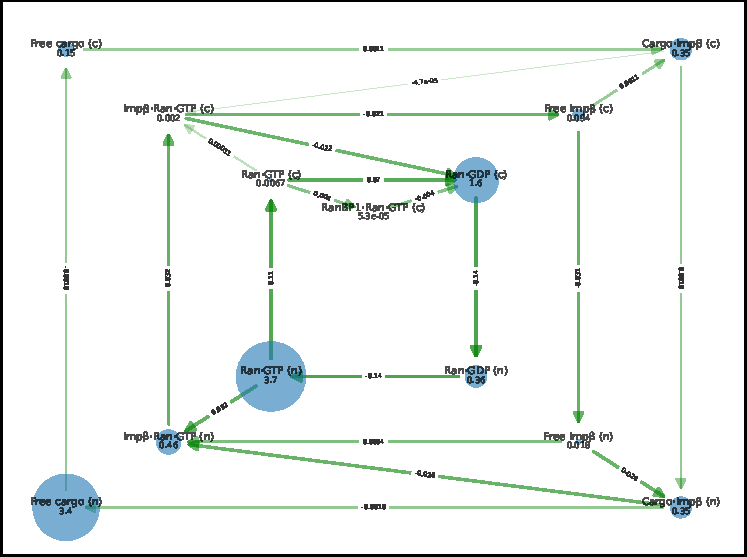
\includegraphics[width=0.7\textwidth]{20210225-GSR/v2/python/b_graph1/onion}
\caption{%
	Steady-state of 
	the transport system from 
	\S\ref{s:GSR03:Imp} / Table~\ref{t:GSR-ImpB}
	with conditions 
	of Table~\ref{t:GSR-ImpB-const}.
	%
	The free cargo
	shows a 20-fold accumulation
	in the nucleus.
	%
	Units are \si{\micro M} for species
	and \si{\micro M . s^{-1}} for fluxes.
	%
	Initial conditions:
	$[\ce{Ran . GDP}]_\text{cyt} = \SI{5}{\micro M}$,
	$[\ce{Imp$\beta$}]_\text{cyt} = \SI{1}{\micro M}$,
	$[\ce{Cargo}]_\text{cyt} = \SI{3}{\micro M}$,
	all else zero.
}
\label{f:GSR-v2}
\end{figure}



%%% BIBLIOGRAPHY %%%
\clearpage
\printbibliography % biblatex
\normalsize




%\clearpage

\SHOWTODOS
%\TODO{are the stars correct?}
%\TODO{acknowledgements, first footnote}
%\TODO{review the references section}
%\TODO{check name spelling (authors and footnote)}


\leavevmode\vfill{\tiny\color{lightgray}\hfill{\DTMnow}}
\end{document}
